\documentclass[supercite]{HustGraduPaper}
%进行个人信息设置
\title{AI+计算机的可能创新途径的分析} %论文题目
\author{王李超} %作者姓名
\date{\today} %日期,默认当日
\school{计算机科学与技术学院} %院系名称
\classnum{计算机科学与技术专业启明2401} %专业班级
\stunum {U202414887} %学号
\instructor{雷鑑铭} %指导教师姓名

%添加自己要用的其他宏包
\usepackage{xltxtra}
\usepackage{bm}

\begin{document}
	%生成标题页 
	\maketitle[line length=16em]
	%可选参数:
	% logo color=green/black 华中科技大学字样的颜色,绿色或者黑色,默认绿色
	% line length=16em 填写信息处横线的长度,默认12em
	% line font=huawenzhongsong 填写信息的字体,默认huawenzhongsong
	% \maketitle
	
	%生成声明与授权书页 \statement[可选参数]
	%可选参数:
	%confidentiality=yes/no/true/false/empty 是否保密,yes/true为保密;no/false为不保密,empty为不填,默认为empty
	%year=5 保密年数,默认为空
	% \statement
	
	\clearpage %结束上一页
	\pagenumbering{Roman} %摘要页码为大写罗马数字
	
	%填写中文摘要内容和关键字
	\begin{cnabstract}{人工智能;编程;创新}
		2020年,ChatGPT的问世标志着人工智能发展的重要里程碑,也被后世称为“AI元年”。随着AI技术的快速演进,大模型的应用领域从语言生成扩展到视频生成(如Sora)、编程辅助(如Copilot)和图片生成(如MidJourney)等多个方向。作为计算机科学与技术专业的学生,我深刻体会到AI工具在学习与实践中的重要作用。然而,AI在编程领域的潜力远不止于代码生成和调试。本论文从理论角度出发,探讨AI在编程中的创新应用场景与可能的实现方法,包括代码优化、算法改进及架构设计的智能化支持。本文旨在展望AI技术未来的发展方向,并为推动计算机科学的进步提供参考。
	\end{cnabstract}
	%填写英文摘要内容和关键字
	\begin{enabstract}{AI;programming;innovation}
		The emergence of ChatGPT in 2020 marked a pivotal milestone in the evolution of artificial intelligence, earning it the title "Year of AI." With the rapid advancement of AI technologies, large models have expanded their applications beyond language generation to fields such as video creation (e.g., Sora), programming assistance (e.g., Copilot), and image generation (e.g., MidJourney). As a computer science student, I have witnessed the growing impact of AI tools in both learning and practice. However, the potential of AI in programming extends far beyond code generation and debugging. This paper explores theoretical perspectives on innovative applications of AI in programming, including code optimization, algorithm enhancement, architectural design, and intelligent project management. The study aims to envision future directions for AI development while contributing insights to the progress of computer science.
	\end{enabstract}
	
	%生成目录 \tableofcontents[可选参数]
	%可选参数:
	%pagenum=yes/no/true/false 目录是否显示页码,默认为false
	%toc in toc=yes/no/true/false 目录中是否有目录及其页码,默认为false
	%level=4 目录级数,默认是4,即显示到subsubsubsection
	%section indent=0em 目录第一级的缩进,默认是0em
	%subsection indent=1.5em 目录第二级的缩进,默认是1.5em
	%subsubsection indent=3.8em 目录第三级的缩进,默认是3.8em
	%subsubsubsection indent=7em 目录第四级的缩进,默认是7em
	%paragraph indent=11em 目录第五级的缩进,默认是11em
	%subparagraph indent=13em 目录第六级的缩进,默认13em
	%indent=normal/noindent/hustnoindent/sameforsubandsubsub 快速缩进设置,具体见文档
	%dot sep=4.5 目录点间距,默认4.5
	%section dot sep=4.5 目录第一级的点间距,默认是4.5
	%subsection dot sep=4.5 目录第二级的点间距,默认是4.5
	%subsubsection dot sep=4.5 目录第三级的点间距,默认是4.5
	%subsubsubsection dot sep=4.5 目录第四级的点间距,默认是4.5
	%paragraph dot sep=4.5 目录第五级的点间距,默认是4.5
	%subparagraph dot sep=4.6 目录第六级的点间距,默认是4.5
	%请注意在合适的位置放置\pagenumbering{numstyle}使用新的页码
	\tableofcontents[pagenum=yes]
	
	\clearpage%结束上一页
	\pagenumbering{arabic} %正文页码为阿拉伯数字
	
	%正文内容从这里开始
	\section{代码优化}
		事实上,由于人工智能本身就是编程的结果、代码的呈现,有谚语“解铃还须系铃人”,从这个方面看,AI可能比人类更懂代码也就不足为奇了。以下将从自动化性能优化、智能资源管理、语义级别的代码重构三个方面具体探讨。
	% \par 也可以通过\verb|\par|命令来新起一段
	\subsection{自动化性能优化}
		AI在性能优化方面可以通过深度学习模型和静态分析工具的结合,自动发现代码中存在的性能瓶颈。例如,对于复杂的循环结构,AI可以分析每次迭代的时间复杂度,检测是否存在重复计算、内存浪费等问题,进而建议替代方案,如使用缓存(memoization)减少重复计算,或者用矢量化操作加速矩阵运算。对于计算密集型任务,AI还能够识别适合并行化的部分,通过生成多线程或多进程的实现来提升性能。此外,AI还能动态调整算法参数,例如机器学习模型中的超参数,优化性能与资源使用之间的平衡。在大规模分布式系统中,AI还可根据运行时监控信息,实时分析系统的负载分布,优化任务调度策略,减少因资源争用而导致的性能下降。这种自动化的性能优化不仅可以减轻开发者的工作量,还能大幅提高代码在不同场景下的执行效率。
	\subsection{智能资源管理}
	AI在资源管理方面的优化能力主要体现在内存、CPU、GPU等硬件资源的合理分配上。例如,在内存管理中,AI可以通过静态分析预测可能的内存泄漏或高内存占用点,并建议优化策略,如减少不必要的对象分配、改进数据结构的选择等。动态资源管理中,AI能够基于运行时的内存使用情况调整垃圾回收机制,避免内存碎片化或高延迟问题。在多核CPU或GPU加速场景下,AI可以根据任务特性,将计算任务划分为更细粒度的子任务,并自动分配到适当的核心上执行,提升并行效率。在大数据处理环境中,AI可以动态调整数据分片策略、优化I/O操作,避免瓶颈节点的出现。这种基于硬件特性的资源管理优化,可以帮助开发者最大限度地挖掘硬件性能潜力,尤其适用于高性能计算和云计算场景。
	\subsection{语义级别的代码重构}
	AI通过深度学习模型理解代码的功能语义后,可以自动进行代码重构,使代码不仅在功能实现上正确,还符合最佳实践。例如,AI可以识别出存在耦合的代码模块,推荐将其拆分为独立的函数或类,从而提高代码的可维护性和复用性。对于存在冗余逻辑的部分,AI可以通过模式匹配发现重复代码,并建议抽象为通用函数。与此同时,AI还能识别不符合命名规范的变量或函数名称,并建议更具描述性的命名,以提升代码可读性。在重构过程中,AI还会关注性能优化,如将低效的算法逻辑替换为更优的实现。此外,AI还能根据代码历史或团队的开发风格,自动调整代码格式,使整个代码库风格统一,便于协作和审查。这种语义级别的自动化重构,不仅减轻了开发者手动修改代码的负担,还显著提高了软件的质量与可维护性。
	
	% \verb|\subsubsubsection|是本样式定义的第四级标题,其使用方法与前三级相同。
	
	% \paragraph{段落}\label{para:para}这是一个带有顶头标签的段落这是一个带有顶头标签的段落这是一个带有顶头标签的段落这是一个带有顶头标签的段落这是一个带有顶头标签的段落这是一个带有顶头标签的段落这是一个带有顶头标签的段落
	% \subparagraph{小段落}\label{subpara:subpara}只是一个带有缩进标签的段落只是一个带有缩进标签的段落只是一个带有缩进标签的段落只是一个带有缩进标签的段落只是一个带有缩进标签的段落只是一个带有缩进标签的段落只是一个带有缩进标签的段落
	\section{算法改进}
	\subsection{现有经典算法的启发}
	许多人类设计的经典算法具有深远影响。例如:
	\par {\songti \bfseries 排序算法:}如快速排序(QuickSort),其基于分治思想在实际应用中表现出卓越的时间效率。
	\par {\songti \bfseries 图算法:}如Dijkstra算法,解决了单源最短路径问题,并广泛应用于导航和网络路由。
	\par {\songti \bfseries 搜索算法:}如A*算法,结合了启发式搜索和代价函数,是路径规划领域的核心算法。
	\par {\songti \bfseries 机器学习算法:}如支持向量机(SVM)和随机森林,这些算法在人类精心设计的基础上实现了分类和回归任务的高效解决方案。
	\par 尽管这些算法已经非常成熟,但它们也存在改进空间。例如,Dijkstra算法在稀疏图中效率较低,A*算法的性能依赖于启发函数的质量,而QuickSort在数据接近有序时表现不佳。

	\subsection{AI在改进算法中的角色}
	AI可以通过以下几个途径在算法设计与改进中发挥作用:
	\subsubsection{\songti \bfseries 基于深度学习的启发式优化}
启发式算法在解决复杂问题时表现优越,其关键在于启发式函数的设计质量。然而,传统启发式函数往往依赖于开发者的经验和对问题的理解,难以达到通用性和高效性兼顾的目标。AI的深度学习技术为优化启发式函数提供了全新途径。

以A算法为例,其效率高度依赖于启发式函数的准确性。传统的启发式函数(如欧几里得距离或曼哈顿距离)通常无法针对特定场景提供最佳估计。通过深度学习技术,AI可以从大量历史数据中学习更加精准的启发式函数。例如,在一个动态地图环境中,AI可以利用卷积神经网络(CNN)分析地图特征,根据地图中的障碍分布和路径选择模式,生成对目标距离更贴近实际的估计值。这样的改进能够显著减少A算法的搜索节点数量,从而提高效率。

除了路径搜索,深度学习在优化其他启发式算法的评估策略方面也有重要潜力。例如,在旅行商问题(TSP)中,AI可以通过图神经网络(GNN)学习城市间距离的特定特征,从而生成适合特定场景的启发式规则。这种规则能够有效减少算法在解空间中的探索次数,提高求解效率。

深度学习优化启发式函数的优势在于其动态适应性和场景感知能力。与传统静态规则相比,AI生成的启发式函数能够根据应用场景的变化实时调整,使算法在不同环境下都能保持优异性能。这种创新方式不仅推动了启发式算法的发展,也为解决复杂优化问题提供了新的工具和思路。
	\subsubsection{\songti \bfseries 自动化算法结构生成}
	传统算法的设计通常基于开发者的理论推导和经验积累,其效率和适用性依赖于问题本身的特性。然而,AI通过神经架构搜索(NAS)技术,能够突破人类思维的限制,在复杂的搜索空间中自动生成优化的算法结构,为传统算法设计开辟了新的可能性。

以排序问题为例,QuickSort作为经典算法,基于分治思想在大多数场景下表现良好。然而,对于特定类型的数据分布(如高度有序或包含大量重复值的数据),其性能可能不尽如人意。AI可以利用NAS技术,探索更优的数据划分策略与比较方法。例如,AI可以结合历史数据分析和深度强化学习,尝试不同的划分点选择规则(如结合数据统计特性的动态划分)和排序优化策略(如多线程并行排序或结合缓存优化的局部排序)。在搜索过程中,AI能够通过评估不同策略的性能,不断改进算法结构,最终生成在特定场景下效率更高的新型排序算法。

这种方法的优势在于,AI不仅能够优化现有算法的结构,还能探索传统设计范式以外的可能性。例如,对于图算法中的最短路径问题,AI可以结合NAS技术生成全新的搜索策略,适应复杂图结构或实时变化的边权重。

通过自动化算法结构生成,AI使算法设计从经验驱动转变为数据驱动和智能探索。开发者无需深入理解复杂理论,只需提供问题定义和目标条件,AI便可生成适合的算法。这种技术在加速算法开发的同时,也为解决更多实际问题提供了灵活高效的工具。
	\subsubsection{\songti \bfseries 混合算法的创新性融合}
	传统算法通常具有固定的设计框架,优点和缺点相对明显。然而,不同算法的特性往往在特定场景中可以形成互补。AI通过分析这些特性,能够生成结合多种优点的新型混合算法,从而在广泛的应用场景中实现更优性能。

以图算法中的最短路径问题为例,Dijkstra算法以其确定性和稳定性著称,但在处理稀疏图或大规模图时,计算效率较低。而A*算法通过引入启发式函数,大幅提升了搜索效率,但其性能依赖于启发式函数的设计质量。AI可以结合两者的特点,生成一种动态调整启发式的混合算法。例如,对于稀疏图,AI可能更倾向于启发式搜索以减少搜索空间;而在密集图中,AI可以优先采用Dijkstra的方式避免不必要的估计误差。通过实时调整,混合算法能够在不同图结构下都表现出色。

此外,AI还可以在其他领域实现算法的融合创新。例如,在优化问题中,遗传算法的全局搜索能力与粒子群优化的快速收敛特性各有优势。AI可以分析两者的性能,在不同搜索阶段动态调整权重,生成一种更加智能的混合算法,既保留全局搜索的能力,又提高收敛速度。

这种混合算法的生成依赖于AI对不同算法特性的大量学习和模拟。通过历史数据和仿真分析,AI能够识别不同算法的强项和短板,并基于特定问题的需求权衡这些特性。相比于传统的单一算法,这种融合方式大幅提高了算法的适应性和通用性,使其能够在更加多样化的场景中提供高效解决方案。
	\subsubsection{\songti \bfseries 针对硬件优化的算法设计}
	现代硬件的发展为算法优化提供了新的可能性,但传统算法设计往往未充分考虑硬件特性,导致性能无法完全发挥。AI通过对硬件特性的深度理解,可以生成更加贴合硬件特性的算法,从而在性能上实现突破。

以矩阵乘法为例,这是一种在深度学习和科学计算中被广泛使用的基本操作。传统的矩阵乘法算法在通用硬件上表现良好,但对于GPU或TPU等专用硬件,其性能仍有优化空间。AI可以通过分析硬件的内存访问模式和计算特点(如并行计算能力和缓存结构),自动调整矩阵分块策略,优化线程调度和数据加载方式。例如,对于大规模矩阵,AI可能会设计出多级分块算法,使得数据在缓存中复用率更高,从而减少内存访问时间。

除了矩阵乘法,AI还可以优化其他与硬件强相关的算法。例如,在图像处理领域,AI可以结合GPU的并行能力,生成适合大规模图像处理任务的卷积优化算法。这种算法不仅能够提高计算速度,还能降低硬件功耗,提升整体效率。

通过针对硬件优化的算法设计,AI能够帮助开发者充分发挥现代硬件的性能潜力。随着硬件技术的不断进步,AI将在算法与硬件之间架起更紧密的桥梁,推动软件性能迈上新的台阶。
	\subsubsection{\songti \bfseries 动态适应性的算法改进}
	传统算法通常是静态的,其参数和执行策略在设计阶段便已确定。这种方式虽然简单,但难以适应运行时环境的变化。AI通过引入动态适应性,可以使算法根据实时数据调整行为,从而在多变的场景中始终保持高效。

遗传算法是一种典型的优化算法,其性能依赖于参数的选择(如种群规模、交叉概率和变异概率)。在传统实现中,这些参数通常是固定的,导致算法在不同问题或阶段的表现存在局限性。AI可以开发出一种动态遗传算法,根据实时数据动态调整参数。例如,在早期搜索阶段,AI可以增加变异概率以增强全局探索能力;而在后期搜索阶段,AI可以降低变异概率以加速收敛。这种动态调整使得算法能够更高效地找到最优解。

此外,在实时系统中,动态适应性尤为重要。例如,在流量调度问题中,网络流量可能会随着时间和需求的变化而波动。AI可以开发一种动态负载均衡算法,实时分析网络流量分布并调整流量调度策略,从而确保网络的高效运行和服务质量。

通过动态适应性的改进,AI为传统算法注入了更多灵活性和智能化特性。这种改进不仅扩展了算法的应用范围,还提升了其在复杂环境中的表现能力。

	\section{架构设计}
	\subsection{自动化生成架构设计}
 AI的自动化能力可以显著改变架构设计的传统方式。借助自然语言处理(NLP)技术,AI能够将开发者或业务人员提出的需求描述转化为系统架构的初步设计。例如,用户只需用自然语言表达需求,如“我们需要一个社交媒体平台,包含用户注册、好友添加、信息发布和实时聊天功能。”AI就可以通过分析这些关键词,自动生成一个初步的架构蓝图。该蓝图可能包括前后端分离的设计,前端部分处理用户界面和交互逻辑,后端部分负责数据管理和业务逻辑。

此外,AI可以根据项目的规模和功能需求,建议适合的技术栈。例如,对于需要高性能和快速响应的实时聊天功能,AI可能会推荐使用Node.js和WebSocket技术;而对于数据存储,它可能建议使用MongoDB来处理非结构化数据。这些推荐不仅基于当前的技术趋势,还可以结合行业经验和最佳实践。例如,AI可能会提示开发者在微服务架构中为每个功能模块(如用户管理、信息发布)设计独立的服务,以便后期更容易扩展或维护。

进一步地,AI还可以提供更详细的设计,例如定义模块间的接口和通信方式,甚至生成数据库的初步设计。举例来说,AI可能会建议设计一张用户表用于存储注册信息,同时提醒开发者为密码字段加密,增强安全性。此外,AI还能指出潜在的设计问题,比如某个模块过于复杂可能会导致后期维护困难,并提供优化方案。这种能力尤其适合初学者或小型团队,他们可以通过AI的指导,快速完成从需求到架构设计的转化过程。

通过自动化生成架构设计,AI不仅可以大幅节省时间,还能降低人为错误的风险,同时提升设计的规范性和可扩展性。对于那些缺乏经验的开发者来说,这种工具更是有助于弥补知识的空白,让他们能够设计出高质量的系统。
     \subsection{数据驱动的架构优化}
传统的架构优化往往依赖开发者的经验和直觉,而AI能够基于数据分析提供更精准和高效的优化方案。现代软件系统的运行会生成大量数据,包括用户访问量、服务响应时间、系统错误率等。AI可以利用这些数据,识别出系统中的性能瓶颈,并提出具体的优化建议。例如,在一个基于微服务架构的电商平台中,AI可能会发现某个服务的响应时间比其他服务长,从而定位问题可能出现在该服务的数据库查询效率上。AI可以建议开发者使用索引优化查询,或者在缓存中存储常用数据以减少数据库负载。

除了定位瓶颈,AI还可以分析系统的整体结构,从中发现可能的优化机会。例如,对于流量分布不均的服务,AI可以建议开发者采用负载均衡策略,避免某些服务因流量过大而导致延迟甚至崩溃。AI还能结合历史数据和预测模型,分析系统的扩展能力,提醒开发者提前为未来的流量增长做好准备,例如拆分单体架构或引入更多的服务实例。

AI的另一个重要作用是学习行业内的最佳实践。例如,它可以分析其他类似系统的架构优化案例,提取有效的优化方法并应用到当前系统中。例如,对于一个内容推荐系统,AI可能会建议使用基于分布式计算的架构,如Hadoop或Spark,以便更高效地处理大规模数据。

通过这些数据驱动的优化方式,AI不仅可以帮助开发者提高系统的性能和稳定性,还能显著降低架构优化的时间和成本。对于那些复杂度较高的大型系统,AI的作用尤为明显,因为它能够快速处理大量的数据,并从中提取人类可能忽略的重要信息。

\subsection{动态架构调整}
在传统的软件开发中,系统架构通常是在开发阶段完成设计,并在上线后很少发生变化。然而,随着需求的变化和用户规模的增长,原本固定的架构可能难以满足实际需求。这时,动态架构调整变得尤为重要,而AI正是实现这一能力的关键工具。

AI可以通过监控系统的实时运行数据,动态调整架构以适应当前的工作负载。例如,在一个直播平台中,访问量可能会因热门直播间的突然涌入而迅速攀升。传统的架构设计可能无法及时应对流量高峰,导致服务中断或响应缓慢。而AI可以通过预测流量峰值,在高峰到来之前自动建议或触发资源扩展,比如增加服务器实例或重新分配现有资源以优先支持直播服务。

在分布式系统中,任务分配策略对系统性能至关重要。AI可以实时分析任务负载,动态调整任务分配。例如,在一个数据处理系统中,如果某些节点的负载过高,AI可以将部分任务转移到负载较轻的节点,避免资源浪费或单点故障。此外,AI还能根据任务的特性(如计算密集型或数据密集型)选择最适合的节点进行处理,进一步提升系统效率。

更先进的是,AI可以通过预测未来的需求变化,提前进行架构调整。例如,在电商平台的促销活动期间,AI可以分析历史数据和当前趋势,预测未来的流量高峰,并在促销开始前调整架构。例如,它可以提前扩展数据库实例数量,提高缓存容量,甚至临时改变系统的服务优先级,以确保核心功能的稳定运行。

通过动态架构调整,AI能够让系统在运行时适应环境和需求的变化。这不仅减少了人为干预的需求,还能显著提高系统的可靠性和用户体验。随着AI技术的进一步发展,这种能力有望成为未来软件系统的标配,使系统能够在复杂多变的环境中始终保持最佳状态。
	% 本模板已经引入伪加粗和伪斜体,这样就不需要对应的粗体和斜体字体也能生成需要的效果,就像下面这样
	
	% {\songti \bfseries 宋体加粗}
	
	% {\songti \itshape 宋体斜体}
	
	% {\songti \bfseries \itshape 宋体粗斜体}
	
	% 请注意,使用加粗和斜体时,请与字体名称一同使用,否则会自动将粗体匹配为黑体,斜体匹配为楷体,就像下面这样
	
	% {正常显示宋体}
	
	% {\bfseries 加粗后变为黑体}
	
	% {\itshape 斜体后变为楷体}
	
	% \section{新的大节}
	% 新的大节会自动出现在新的一页上
	% \section{参考文献和交叉引用}\label{sec:ref}
	% \subsection{参考文献}
	% 这是一个参考文献引用的范例\cite{Stone_1998},你可以随时使用两种不同的样式\normalcite{Stone_1998}或者\supercite{Stone_1998}
	
	% 这样可以添加一个不标注的参考文献引用\nocite{9787508342894}
	
	% 这样可以添加所有bib文件中的参考文献\nocite{*}
	
	% \subsection{交叉引用}\label{subsec:crossref}
	% 本模板已经重写了hyperref宏包的\verb|\autoref|命令,方便引用章节、公式和图表。
	
	% 比如说\autoref{sec:ref}和\autoref{subsec:crossref}就引用了本章节,\autoref{para:para}和\autoref{subpara:subpara}引用了之前的两个段落。显然段落因为没有序号,引用结果和上一节的需要相同,因此建议使用段落“\nameref{para:para}”和段落“\nameref{subpara:subpara}”。
	
	% 本样式定义的第四级标题也可以引用,就像这样:\autoref{subsubsubsec:subsubsubsec}。
	
	
	
	% \section{公式这么用}
	% 在文中引用公式可以这么写:$a^2+b^2=c^2$这是勾股定理,他还可以表示为$c=\sqrt{a^2+b^2}$,还可以让公式单独一段并且加上编号
	% \begin{equation}
	% \sin^2{\theta}+\cos^2{\theta}=1 \label{eq:pingfanghe}
	% \end{equation}
	% 还可以通过添加标签在正文中引用公式,如式~\eqref{eq:pingfanghe}~或者\autoref{eq:pingfanghe}。我们还可以轻松打出一个矩阵
	% \begin{equation}
	% \bm{A}=\begin{bmatrix}
	% 1&2&3&4\\
	% 11&22&33&44\\
	% \end{bmatrix}
	% \times\begin{bmatrix}
	% 22&24\\
	% 32&34\\
	% 42&44\\
	% 52&54\\
	% \end{bmatrix}
	% \end{equation}
	% 或者多个带编号的公式
	% \begin{eqnarray}
	% f_1(x)=12x^2+36x+\sin x\\
	% f_2(x)=\sqrt{3}{x^3+3x}
	% \end{eqnarray}
	% 以上
	
	% \section{用图和表的示例}
	% \subsection{图的使用}
	% \XeLaTeX 环境下可以使用EPS、PDF、PNG、JPEG、BMP格式的图片,当然也可以用绘图包直接在\LaTeX 中绘制图形,推荐使用宏包tikz。图的环境是figure,但figure环境使用复杂且不自带标题,因此本模板定义了一个通用版本的generalfig,该环境会将figure内的图片居中并设置标签与引用名,同时会让图片位置设置为所有可行位置(htbp,即此处、页顶、页底、独立一页),此选项可以作为可选参数设置。
	
	% 其使用方法如下:
	
	% \begin{generalfig}[htb]{大数据信息处理框架}{fig:data}
	% 	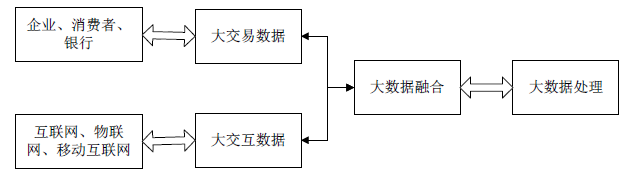
\includegraphics[width=\textwidth]{Figures/data.png}
	% \end{generalfig}
	
	% 同时也可以引用该图片例如:\autoref{fig:data}。请注意generalfig第一个参数是标题,第二个参数是引用。
	
	% \newpage
	
	% \subsection{表的使用}
	% 作为论文,推荐使用三线表进行排版。所谓三线表,即在标题前有横线,标题后有横线,表格最后还有横线,其他地方无线。当然这不是死规定,也可以根据需要在合适的地方加线。
	
	% 本文定义了新的可变长度左中右(LCR)格式,LCR三个格式会根据表格宽度的设定自行控制宽度,且其宽度相等,方便设置和页面相同宽度的表格。但该功能需要使用tabularx做表。
	% \begin{generaltab}{某校学生升高体重样本}{tab:heightweight}
	% 	\begin{tabularx}{\textwidth}{lCCC}
	% 		\toprule
	% 		序号&年龄&身高&体重\\
	% 		\midrule
	% 		1&14&156&42\\
	% 		2&16&158&45\\
	% 		3&14&162&48\\
	% 		4&15&163&50\\
	% 		\cmidrule{2-4} %添加2-4列的中线
	% 		平均&15&159.75&46.25\\
	% 		\bottomrule
	% 	\end{tabularx}
	% \end{generaltab}
	
	% 当然你也可以引用表格,就像这样:\autoref{tab:heightweight}。
	
	% \section{列表的使用}
	% 这是一个计数的列表
	% \begin{enumerate}
	% 	\item 第一项
	% 		\begin{enumerate}
	% 			\item 第一项中的第一项
	% 			\item 第一项中的第二项
	% 		\end{enumerate}
	% 	\item 第二项
	% 	\item 第三项
	% \end{enumerate}

	% 这是一个不计数的列表
	% \begin{itemize}
	% 	\item 第一项
	% 	\begin{itemize}
	% 		\item 第一项中的第一项
	% 		\item 第一项中的第二项
	% 	\end{itemize}
	% 	\item 第二项
	% 	\item 第三项
	% \end{itemize}
	%生成参考文献
	%使用方法:\bibliography{参考文件1文件名, 参考文献2文件名, ...}
	% \bibliography{Bibs/mybib}
	
	% \begin{appendices}
	% 	\section{这是第一个附录}
	% 	这里是附录环境,其中的section、subsection、subsubsection已经变为附录的样式,并且会以这种样式加入目录中
	% 	\subsection{附录可以有小节}
	% 	\subsubsection{附录中也可以有小小节}\label{apxsubsubsec:appendix}
	% 	\subsubsubsection{附录中也有小小小节}
	% 	\verb|\autoref|无法识别Appendices环境,引用效果和正文一样,如\autoref{apxsubsubsec:appendix}。所以如果引用附录的话,建议直接使用附录~\ref{apxsubsubsec:appendix}~。
	% \end{appendices}
\end{document}
